\documentclass[11pt]{article}

\usepackage{a4wide}
\usepackage[utf8]{inputenc}
\usepackage[russian]{babel}
\usepackage{graphicx}
\usepackage{amsmath}
\begin{document}
	
	\thispagestyle{empty}
	
	\begin{center}
		\ \vspace{-3cm}
		
		
\includegraphics[width=0.5\textwidth]{msu.eps}\\
		{\scshape Московский государственный университет имени М.~В.~Ломоносова}\\
		Факультет вычислительной математики и кибернетики\\
		Кафедра системного анализа
		
		\vfill
		
		{\LARGE Отчёт по  практикуму:}
		
		\vspace{1cm}
		
		{\Huge\bfseries <<Численные методы.>>}
	\end{center}
	
	\vspace{1cm}
	
	\begin{flushright}
		\large
		\textit{Студент 315 группы}\\
		А.\,В.~Бабаев
		
		\vspace{5mm}
		
		\textit{Руководитель практикума}\\
		к.ф.-м.н., доцент П.\,А.~Точилин
	\end{flushright}
	
	\vfill
	
	\begin{center}
		Москва, 2020
	\end{center}
	
	\newpage
	
	{\vspace*{-2cm} \hspace{-1cm}\bf \Large  1) Постановка задачи и определение параметров.}
	\newline
	\newline
	{\hspace{-0.6cm} Пусть $f(t)$ - некоторая непрерывная функция. Обозначим Фурье-образ данной функции,	 как функцию $F(\lambda)$:}
	\newline
	
	{\[F(\lambda) = \int_{-\infty}^{\infty}f(t)\cdot e^{-i\lambda t}\,dt. \]}
	\newline 
	\newline
	{Где t - действительная переменная, а $\lambda$ - комплексная. Исходные функции:}		
	\newline 
	\[f_1(t) = t^2 e^{-3|t|}, f_2(t)=\frac{t^3+2t}{t^4 + 4t^2 + 4}, f_3(t) = e^{-3t^4}\cos(t), f_4(t) = \begin{cases}
	e^{-t^2}, \quad {|t| \leq 1}\\
	0 \; ,\qquad{|t| > 1}
	\end{cases} \]
	\newline
	\newline
	{\hspace*{-0.4cm}\bf \Large 2) Теоретические сведения. Сущность вычислений.}
	\newline
	\newline
	{\hspace{-0.6cm}\bf Входные данные:}
	\newline
	{\hspace{-0.6cm} На вход подается некоторая функция $f(t)$, её аналитически рассчитанный Фурье-образ этой функции(если требуется), вектор inpLimVec содержащий параметры для оконной функции, шаг дискретизации для $f(t)$  - step, вектор outLimVec содержащий параметры окна вывода. }
	\newline
	\newline
	{\hspace{-0.6cm}\bf Процесс вычисления:}	
	\newline
	{\hspace{-0.6cm} В начале вычислений, пересчитываю шаг дискретизации для равномерной сетки(обозначим a = inpLimVec(1), b = inpLimVec(2)):
	\newline
	\[T = b - a.   \]
	\[N = round(T/step).\]
	\[step_{new} = T/N.\]
	}
	\newline
	{Далее, продлим по периоду T функцию $g(t) = f(t)*h_{a,b}(t)$, где $h_{a,b}(t) -$оконная функция. Выберем набор из N вещественных чисел:}
	\newline
	\[x_n = g(step_{new}\cdot n),(n = 0,1,2,...,N - 1). \]
	\newline
	\newline
	{Применив БПФ к исходному набору чисел, и умножив полученный набор на $step_{new}$, получим N комплексных чисел:}
	\newline
	\[X_n = step_{new} \cdot \sum\limits_{k=0}^{N-1} g(step_{new} \cdot n) \cdot e^{-\frac{2\pi i k n}{N}},(n = 0,1,2,...,N - 1). \]
	\newline
	\newline
	{Данный набор чисел является набором отсчетов частотной области преобразования Фурье. Частотой дискретизации в полученной области будет величина:}
	\newline
	\[\Delta f = \frac{2\pi}{T}.\] 
	
	\newpage
	
	{\vspace*{-2cm} \hspace{-1cm}\bf \Large  3) Аналитические преобразования функций.}
		\newline
	\newline
	{\hspace{-0.6cm}\bf Функция №1:}
	\newline
	\[ f(t) = t^{2}e^{-3|t|}.\]
	
	\[F(\lambda) = \int_{-\infty}^{\infty}t^2 e^{-3|t|} e^{i\lambda t}\,dt.\]
	\newline
	{\hspace{-0.6cm} Так как функция $f(t)$ - четная, то раскладывая экспоненту с мнимой единицей по формуле Эйлера, получим, что интеграл содержащий синус - будет равен нулю. Теперь, оставшийся интеграл, будем рассматривать только на положительной части числовой прямой. Получим вид: }
	\newline
	\[F(\lambda) = 2\cdot\int_{0}^{\infty}t^2 e^{-3t} \cos(\lambda t )\,dt.\]
	\newline
	{\hspace{-0.6cm} Далее воспользуемся формулой интегрирования по частям $\int_{}^{}fg' = fg - \int_{}^{}f'g$ c подстановкой $f = t^2,  g' = e^{-3t}\cos(\lambda t),  g =\frac{\lambda e^{-3t}\sin(\lambda t) - 3e^{-3t}\cos(\lambda t)}{\lambda^2 + 9}$ получим:}
	\[F(\lambda) = 2t^2\cdot\frac{\lambda e^{-3t}sin(\lambda t) - 3e^{-3t}\cos(\lambda t)}{\lambda^2 + 9}\bigg|_0^\infty - 4\cdot\int_{0}^{\infty}t\cdot\frac{\lambda e^{-3t}\sin(\lambda t) - 3e^{-3t}\cos(\lambda t)}{\lambda^2 + 9}\, dt.\]
	\newline
	{\hspace{-0.6cm} Подставив пределы интегрирования, получим, что первый член в данном равенстве равен нулю. Упростим и разобьем на два интеграла:}
	\newline
	\[F(\lambda) = \frac{-4}{\lambda^2 + 9}(\int_{0}^{\infty}\lambda te^{-3t}\sin(\lambda t)\,dt - \int_{0}^{\infty}3te^{-3t}\cos(\lambda t)\,dt).\]
	\newline
	{\hspace{-0.6cm} Сначала вычислим интеграл содержащий синус. Проинтегрируем его по частям где: \newline    
	$f = t, g' = e^{-3t}\sin(\lambda t), g = \frac{-3 e^{-3t}\sin(\lambda t) - \lambda e^{-3t}cos(\lambda t)}{\lambda^2 + 9}$. При подстановке пределов, первый член будет равным нулю, и останется интеграл:}
	\newline
	\[\int_{0}^{\infty}\frac{-3 e^{-3t}\sin(\lambda t) - \lambda e^{-3t}\cos(\lambda t)}{\lambda^2 + 9}\,dt.\]
	\newline
	{\hspace{-0.6cm} Преобразуем:}
	\newline
	\[\frac{-3}{\lambda^2 + 9}\int_{0}^{\infty}e^{-3t}\sin(\lambda t)\,dt - \frac{\lambda}{\lambda^2 + 9}\int_{0}^{\infty}e^{-3t}\cos(\lambda t)\,dt.\]
	\newline
	{\hspace{-0.6cm} Теперь вычислим:}
	\[\int_{0}^{\infty}e^{-3t}\sin(\lambda t)\,dt\]
	\newline
	{\hspace{-0.6cm} Дважды проинтегрируем(с подстановкой пределов) по частям в первый раз с $f = \sin(\lambda t), g' = e^{-3t}$ и второй раз с $f = \lambda \cos(\lambda t), g' = -\frac{e^{-3t}}{3}$:}
	\newline
	\[ \frac{\lambda }{9} - \frac{\lambda^2}{9}\int_{0}^{\infty}e^{-3t}\sin(\lambda t)\,dt.\]
	\newpage
	{\vspace*{-2cm}\hspace{-0.6cm} Исходный интеграл повторяется в правой части выражения, таким образом можно решить уравнение выразив его: }
	\newline
	\[\int_{0}^{\infty}e^{-3t}\sin(\lambda t)\,dt = -\frac{\lambda}{\lambda^2 + 9}.\]
	\newline
	{\hspace{-0.6cm} Теперь вычислим:}
	\newline
	\[\int_{0}^{\infty}e^{-3t}\cos(\lambda t)\,dt.\]
	\newline
	{\hspace{-0.6cm} Как и в случае с синусом, дважды проинтегрировав по частям с $f = \cos(\lambda t), g' = e^{-3t}$ и второй раз с $f = -\lambda \sin(\lambda t), g' = -\frac{e^{-3t}}{3}$ и подставив пределы интегрирования, получим:}
	\newline
	\[-\frac{1}{3} - \frac{\lambda^2}{9}\int_{0}^{\infty}e^{-3t}\cos(\lambda t)\,dt.\]
	\[\int_{0}^{\infty}e^{-3t}\cos(\lambda t)\,dt = \frac{3}{\lambda^2 + 9}.\]
	\newline
	{\hspace{-0.6cm}Следовательно получим, что:}
	\newline
	\[\int_{0}^{\infty}te^{-3t}\sin(\lambda t)\,dt = -\frac{6\lambda}{(\lambda^2 + 9)^2} .\]
	\newline
	{\hspace{-0.6cm} Проделав те же операции, только над интегралом содержащим косинус, получим:}
	\newline
	\[\int_{0}^{\infty}te^{-3t}\cos(\lambda t)\,dt = \frac{\lambda^2 - 9}{(\lambda^2 + 9)^2}.\]
	\newline
	{\hspace{-0.6cm} Подставим найденные интегралы в начальное выражение и упростим его. Искомый интеграл будет иметь вид:}
	\newline
	\[F(\lambda) =-\frac{36(\lambda^2 - 3)}{(\lambda^2 + 9)^3}. \]
	{\hspace{-0.6cm}\bf Функция №2:}
	\newline
	\[ f(t) = \frac{t}{t^2 + 2}.\]
	\[F(\lambda) = \int_{-\infty}^{\infty}\frac{t}{t^2 + 2} e^{i\lambda t}\,dt.\]
	\newline
	{\hspace{-0.6cm} Так как функция $f(t)$ - нечетная, то часть интеграл содержащий косинус будет равным нулю. Останется.}
	\newline
	\[F(\lambda) = i\cdot\int_{-\infty}^{\infty}\frac{t\sin(\lambda t)}{t^2 + 2}\,dt.\]
	\newline
	\[\int_{-\infty}^{\infty}\frac{t\sin(\lambda t)}{t^2 + 2}\,dt = \int_{-\infty}^{\infty}\frac{t\sin(\lambda t)}{(t - \sqrt{2}i)(t+\sqrt{2}i)} = \frac{1}{2}\int_{-\infty}^{\infty}\frac{\sin(\lambda t)}{t + \sqrt{2}i}\,dt + \int_{-\infty}^{\infty}\frac{\sin(\lambda t)}{t - \sqrt{2}i}\,dt. \,\,\,\,\,(*)\]
	
	\newpage
	{\vspace*{-2cm} \hspace{-0.6cm} Вычислим первый из интегралов:}
	\newline
	\[\int_{-\infty}^{\infty}\frac{\sin(\lambda t)}{t + \sqrt{2}i}\,dt =\{u = t + \sqrt{2}i, \frac{du}{dt}=1\} = \int_{0}^{\infty}\frac{\sin(\lambda u - \sqrt{2}i\lambda)}{u}\,du. \]
	\newline
	{\hspace{-0.6cm} Разложим синус по формуле разности аргументов:}
	\newline
	\[\int_{-\infty}^{\infty} \frac{cos(\sqrt{2}i\lambda)sin(\lambda u) - sin(\sqrt{2}i\lambda)cos(\lambda u)}{u}\,du = cos(\sqrt{2}i\lambda)\int_{-\infty}^{\infty}\frac{sin(\lambda u)}{u}\,du - sin(\sqrt{2}i\lambda)\int_{-\infty}^{\infty}\frac{cos(\lambda u)}{u}\,du.
	 \]
	 \newline
	 {\hspace{-0.6cm} Интегральный косинус, при таких пределах обращается в нуль, а интегральный синус в $\pi \cdot sgn(\lambda)$.Проделав ту же работу, только уже со вторым членом в (*) и подставив получим ответ:}
	 \newline
	 \[F(\lambda) = i\cdot sgn(\lambda)\pi e^{-\sqrt{2}|\lambda|}. \]
	
	\newpage
	{\vspace*{-2cm} \hspace{-1cm}\bf \Large  4) Графики преобразований и подзадачи.}
	\newline
	\newline
	{\hspace{-1cm} \bf \large Функция  $f_1(t):$}
	\begin{center}
			{a = -10, b = 10, $\Delta t = 0.01.$}
			\newline
			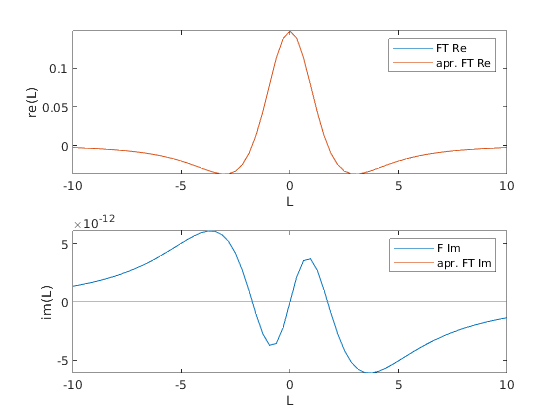
\includegraphics[width=0.8\textwidth]{f1_10_10.png}\\
			
			{a = -100, b = 100, $\Delta t = 0.001.$}
			\newline
			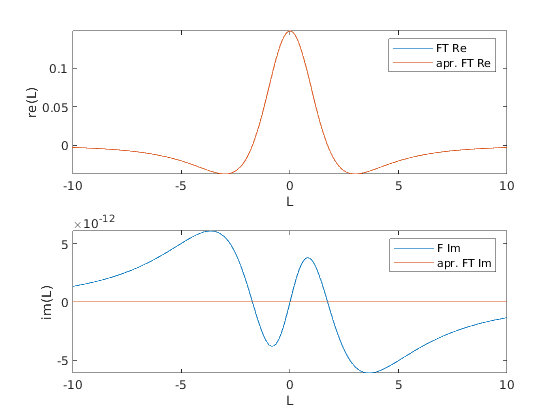
\includegraphics[width=0.8\textwidth]{f1_100_100.png}\\		
	\end{center}
	
	\newpage
	{\hspace{-1cm}\bf \large Функция  $f_2(t):$}
	\begin{center}
		{a = -10, b = 10, $\Delta t = 0.01.$}
		\newline
		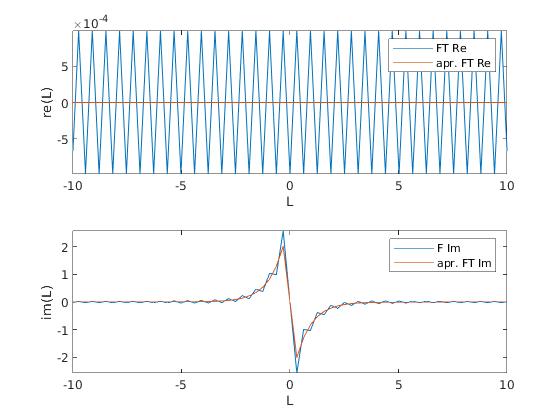
\includegraphics[width=0.8\textwidth]{f2_10_10.png}\\
		{a = -30, b = 30, $\Delta t = 0.001.$}
		\newline
		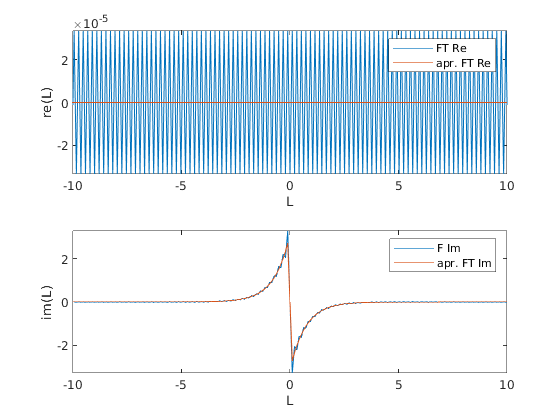
\includegraphics[width=0.8\textwidth]{f2_30_30.png}\\	
	\end{center}
	\newpage
	{\hspace{-1cm}\bf \large Функция $f_3(t):$}
	\begin{center}
		{a = -100, b = 100, $\Delta t = 0.01.$}
		\newline
		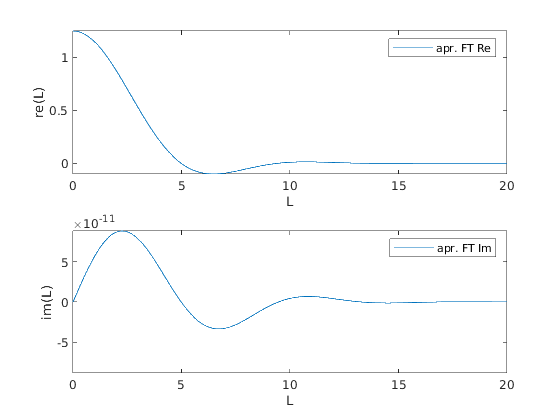
\includegraphics[width=0.8\textwidth]{f3.png}\\
	\end{center}
		{\hspace{-1cm}\bf \large Функция $f_4(t):$}
	\begin{center}
		{a = -100, b = 100, $\Delta t = 0.01.$}
		\newline
		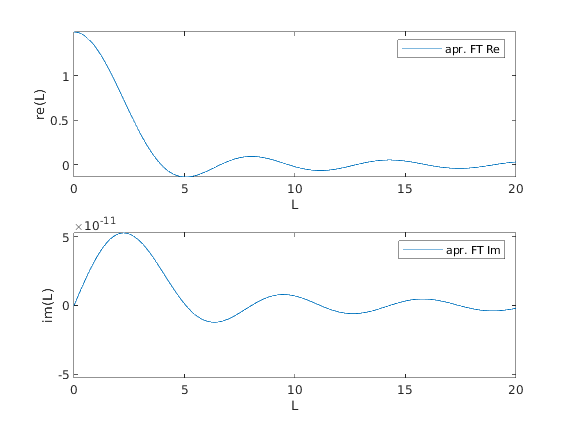
\includegraphics[width=0.8\textwidth]{f4.png}\\
	\end{center}
	\newpage
	{\hspace{-1cm}\bf \large Иллюстрация эффекта наложения спектров и его устранения:}
	\begin{center}
		{Функция $f_2$, a = -100, b = 100, $\Delta t = 0.85$:}
		\newline
		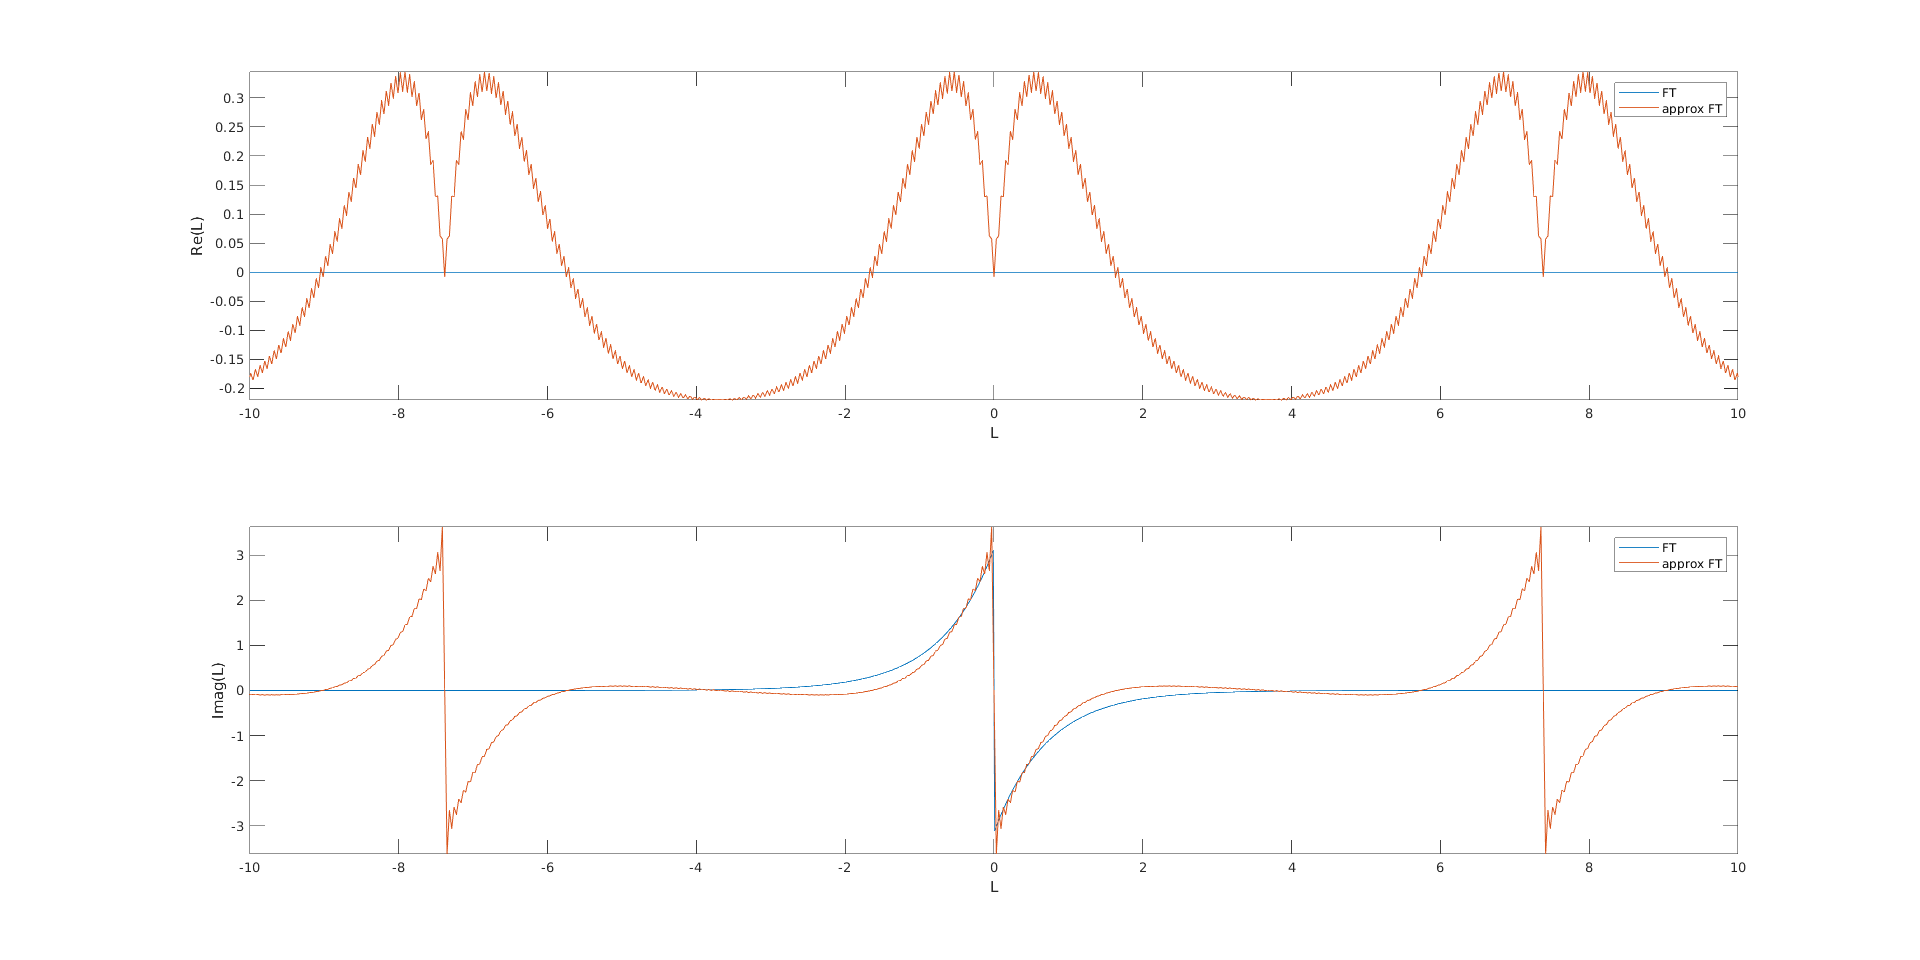
\includegraphics[width=1\textwidth]{nalf_1.png}\\
	
		{Для устранения наложения, в данном случае, можно уменьшить шаг. a = -100, b = 100, $\Delta t = 0.01$:}
		\newline
		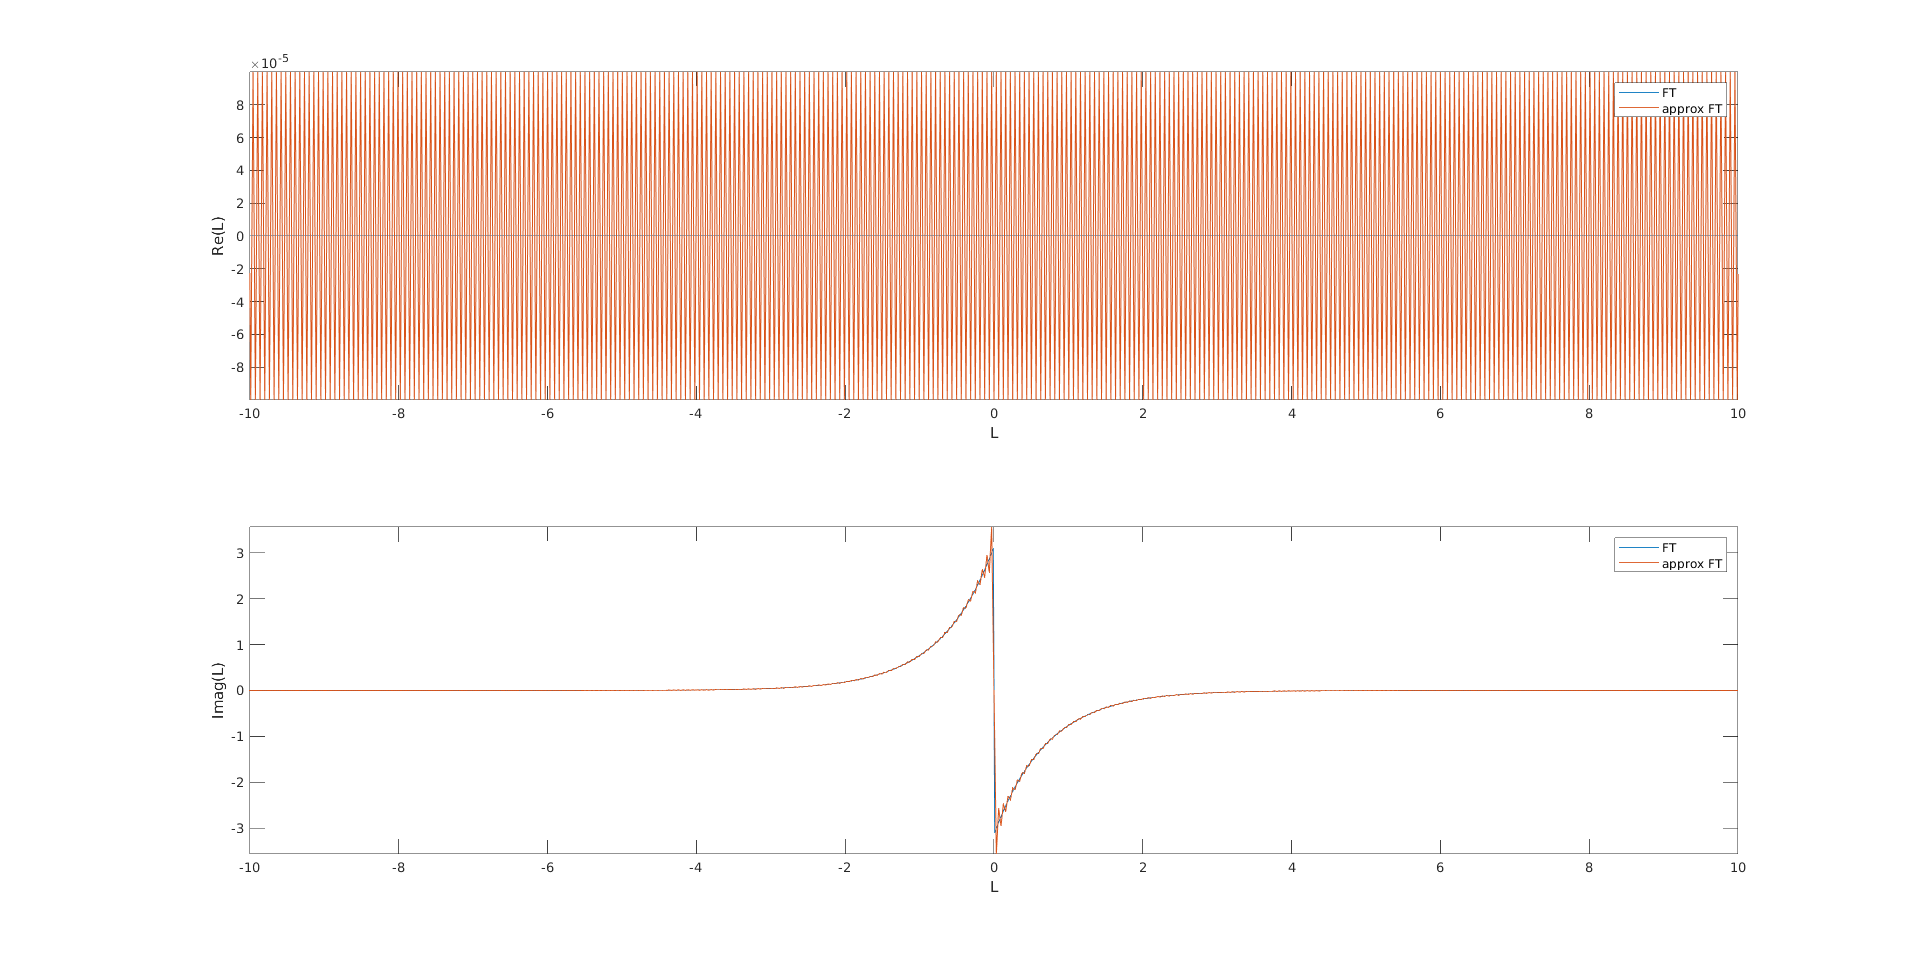
\includegraphics[width=1\textwidth]{nalf_2.png}\\
	\end{center}
	\newpage
	{\hspace{-1cm} \bf Иллюстрация ряби и её возможности устранения:}
	\begin{center}
		{Функция $f_2$, a = -100, b = 100, $\Delta t = 0.05$:}
		\newline
		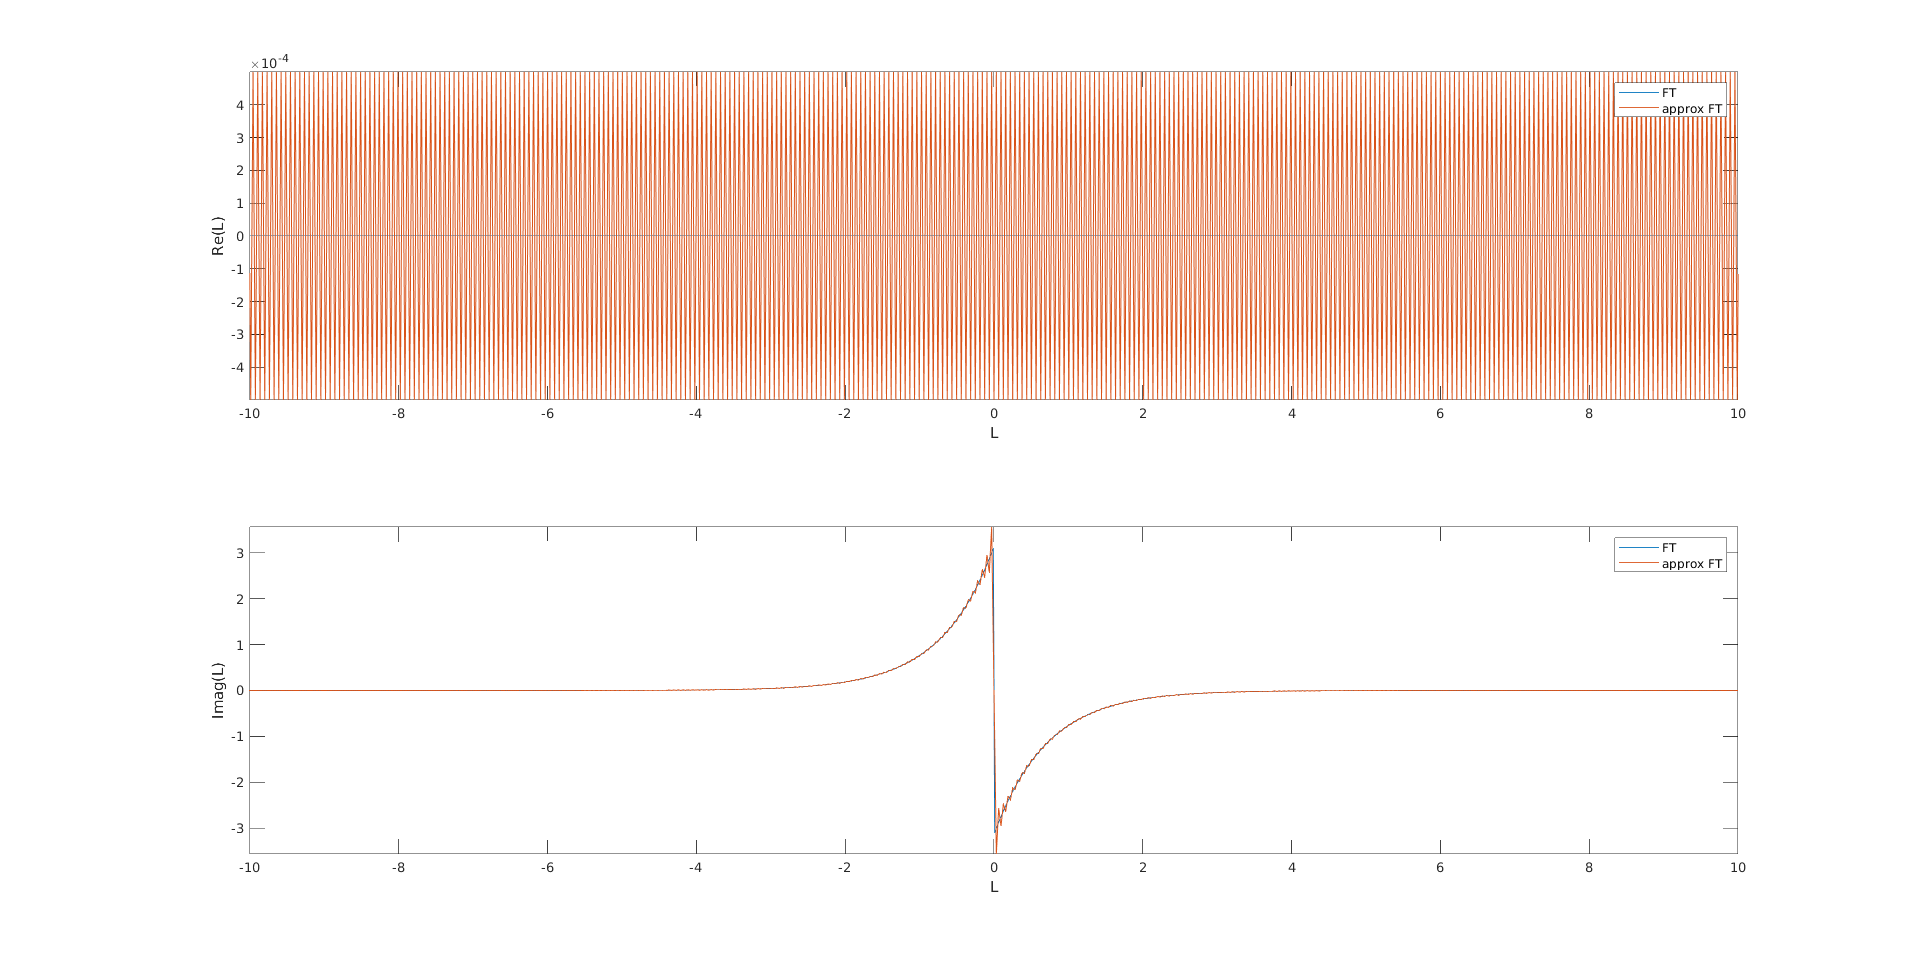
\includegraphics[width=1\textwidth]{ryab_1.png}\\
		{Функция $f_2$, a = -100, b = 100, $\Delta t = 0.0001$:}
		\newline
		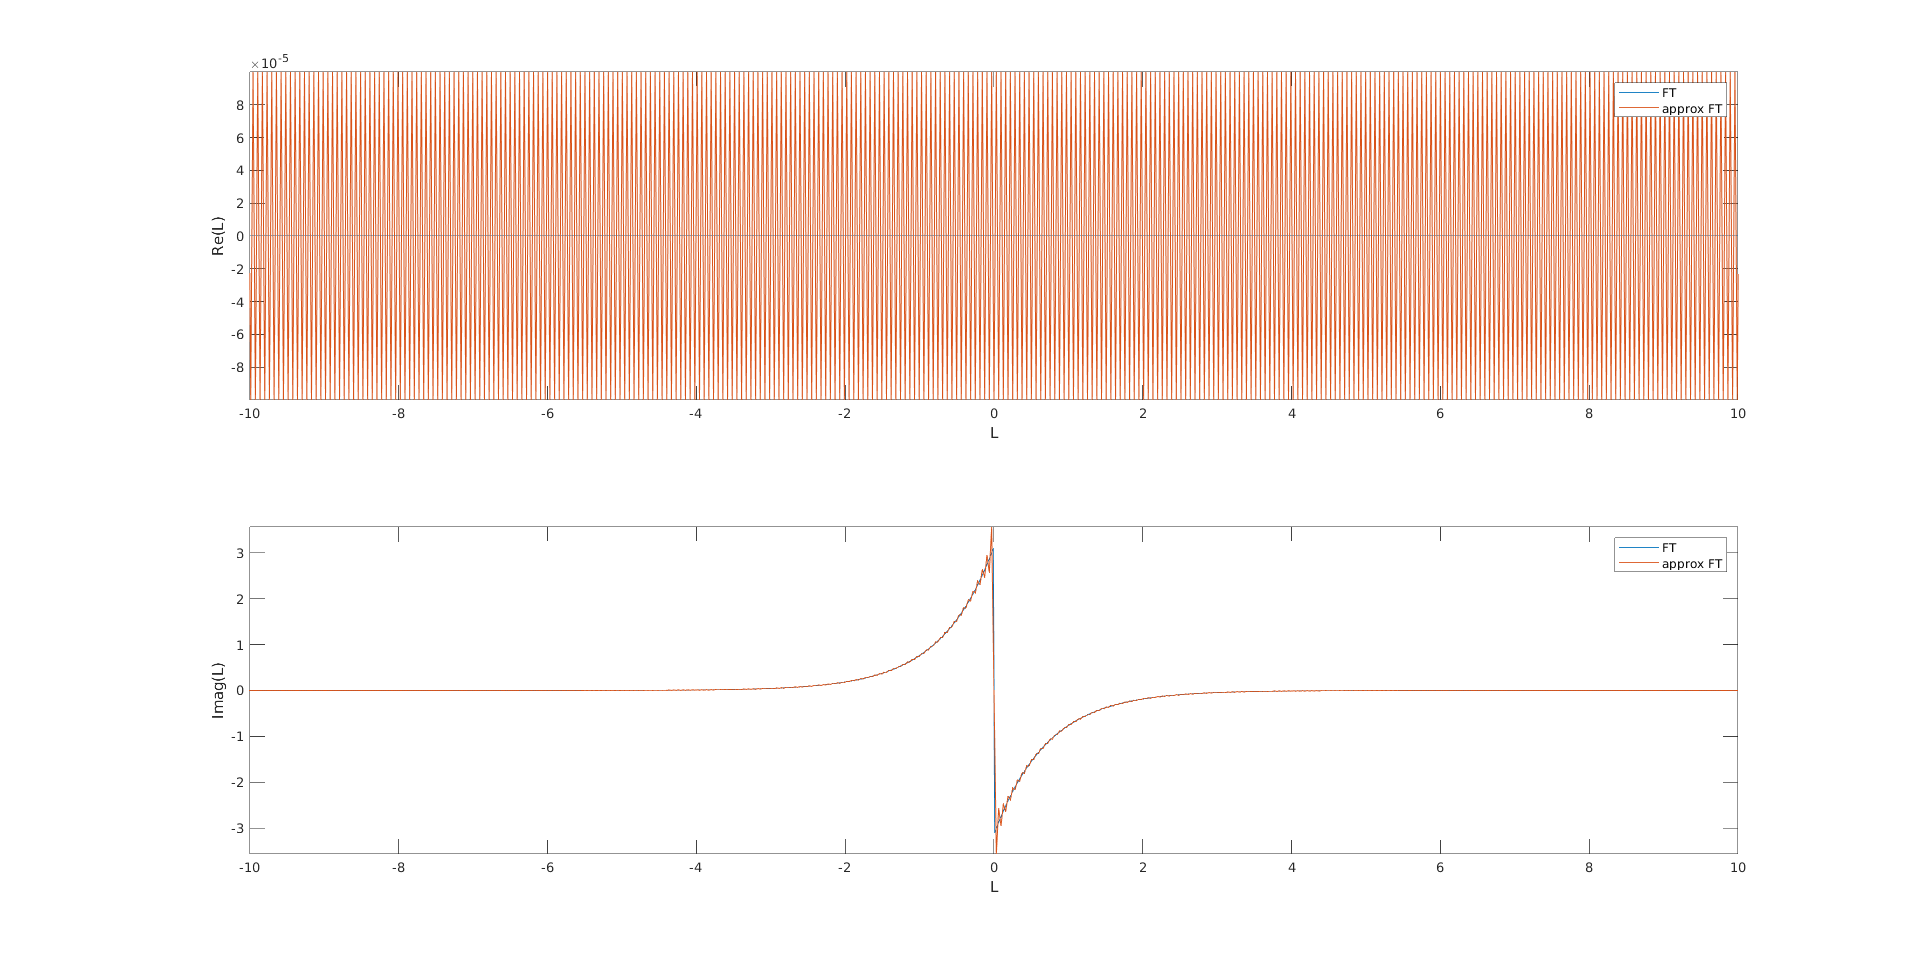
\includegraphics[width=1\textwidth]{nalf_2.png}\\
		{Нижний график демонстрирует невозможность устранения ряби в точке разрыва при "улучшении" параметров.}
	\end{center}		
	\newpage
		{\hspace{-1cm} \bf Устранение ряби, при улучшении параметров:}
	\begin{center}
		{Функция $f_2$, a = -100, b = 100, $\Delta t = 0.01$:}
		\newline
		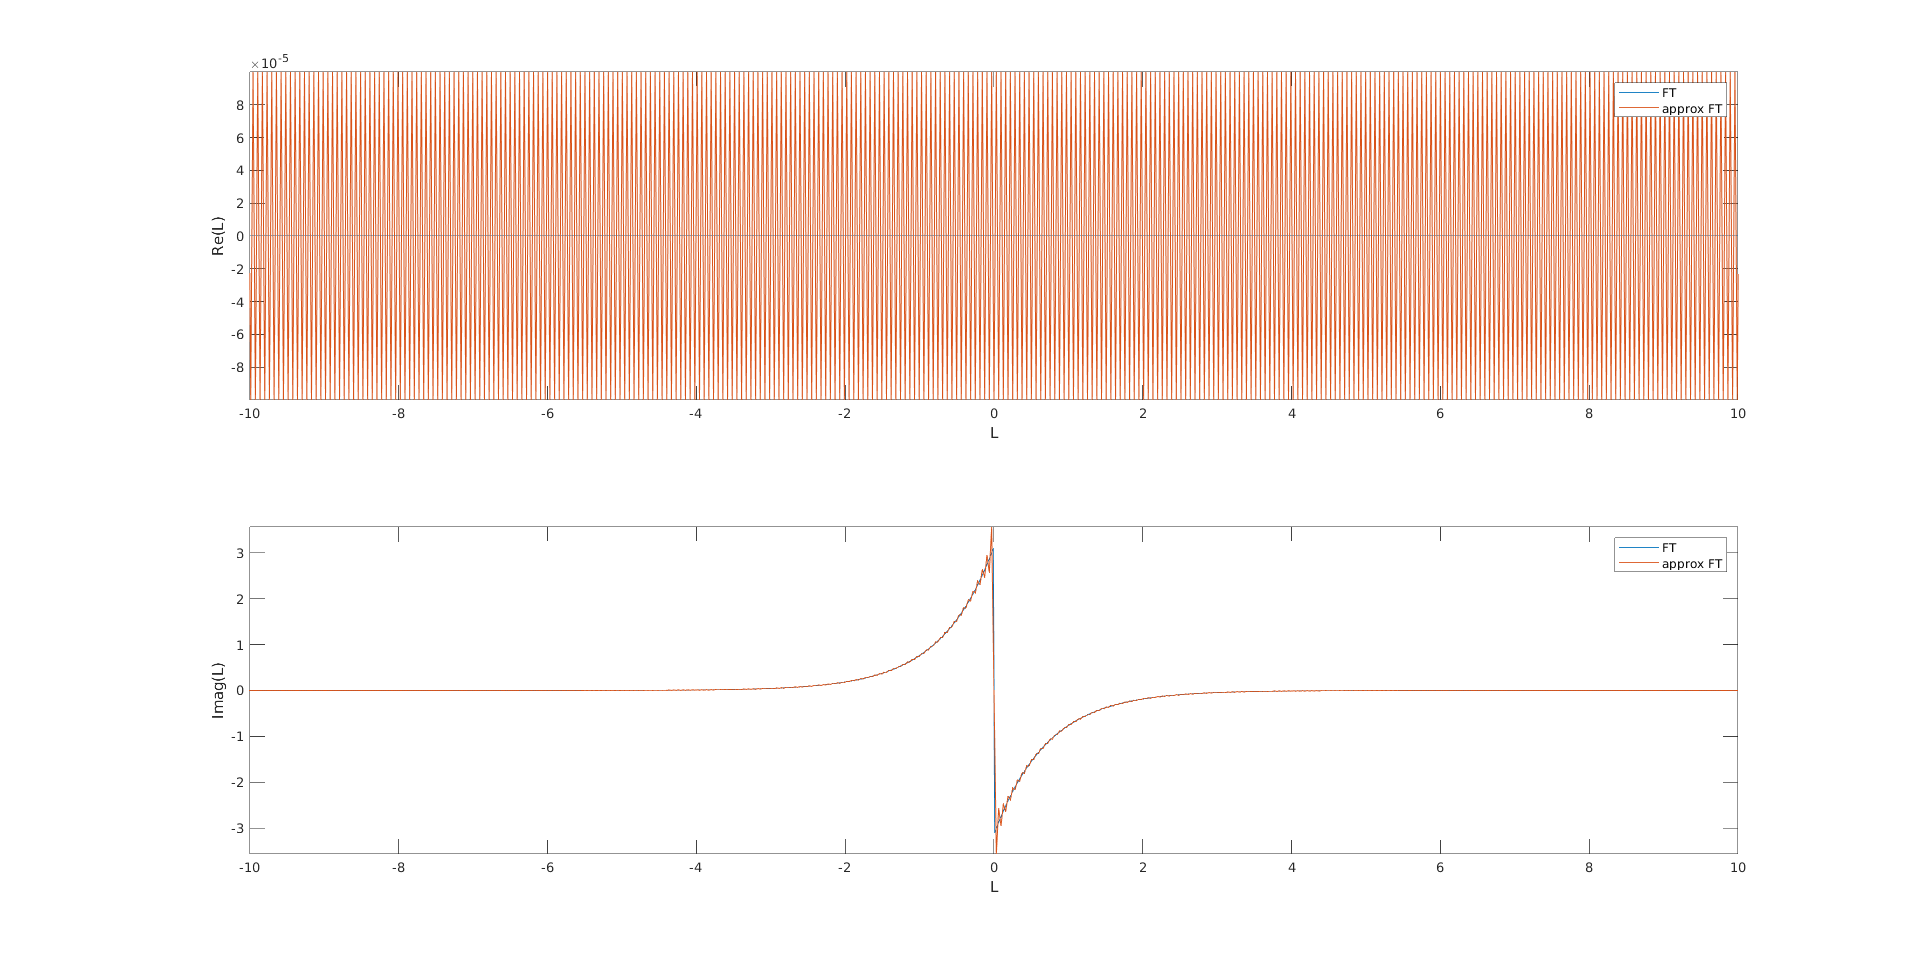
\includegraphics[width=1\textwidth]{r_1.png}\\
		{Функция $f_2$, a = -10, b = 10, $\Delta t = 0.01$:}
		\newline
		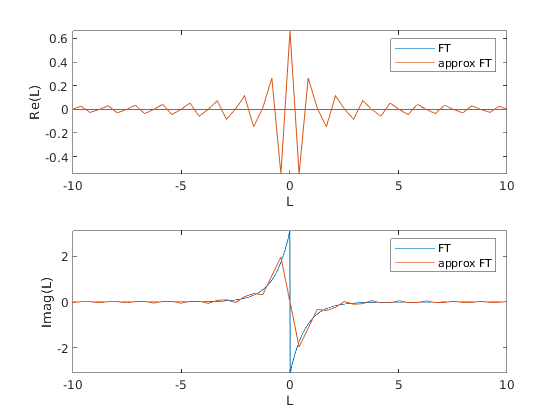
\includegraphics[width=0.8\textwidth]{r_2.png}\\
		{Верхний график демонстрирует возможность частичного устранения ряби, при "улучшении" параметров.}
	\end{center}
\end{document}
